% !TeX spellcheck = <none>
\documentclass[12pt]{report}
%\usepackage[a4paper]{geometry}
\usepackage[right=2.0cm, left=3.5cm, top=2.5cm, bottom=2.5cm]{geometry}
\usepackage[utf8]{inputenc}
%\usepackage{slovak}
\usepackage[slovak]{babel}
\usepackage{epsfig}
\usepackage{color}
\usepackage{url}
\usepackage{amsmath}
\usepackage{amsfonts}
\usepackage{amssymb}
\usepackage{mathtools}
\usepackage{listings}
\usepackage{algpseudocode}
\usepackage{algorithm}
\usepackage{program}
\usepackage{multicol}
\usepackage{framed}
\usepackage{titlesec}
\usepackage{subfig}
\usepackage{textcomp}

\definecolor{gray}{rgb}{0.4,0.4,0.4}
\definecolor{darkblue}{rgb}{0.0,0.0,0.6}
\definecolor{cyan}{rgb}{0.0,0.6,0.6}

\lstset{
  basicstyle=\ttfamily,
  columns=fullflexible,
  showstringspaces=false,
  commentstyle=\color{gray}\upshape
}

\lstdefinelanguage{XML}
{
  morestring=[b]",
  morestring=[s]{>}{<},
  morecomment=[s]{<?}{?>},
  stringstyle=\color{black},
  identifierstyle=\color{darkblue},
  keywordstyle=\color{cyan},
  morekeywords={xmlns,version,type}% list your attributes here
}

\lstset{language=XML}

\renewcommand\baselinestretch{1.5} % riadkovanie jeden a pol 1.3

% pekne pokope definujeme potrebne udaje
\def\mftitle{Vizualizácia verifikácie predpovedných modelov počasia}
\def\mfthesistype{Diplomová práca}
\def\mfauthor{Bc. Marek Kružliak}
\def\mfadvisor{RNDr. Andrej Lúčny, PhD.}
\def\mfplacedate{Bratislava, 2015}
\def\mfprogram{Aplikovaná informatika}

\ifx\pdfoutput\undefined\relax\else\pdfinfo{ /Title (\mftitle) /Author (\mfauthor) /Creator (PDFLaTeX) } \fi

\begin{document}

% obal
\begin{titlepage}
	\begin{minipage}{0.2\textwidth}
	
\includegraphics[width=0.9\textwidth]{komlogo-new.pdf}
	\end{minipage}
	\begin{minipage}{0.8\textwidth}
	\begin{center}
		\sc
		Univerzita Komenského, Bratislava \\
		Fakulta Matematiky, Fyziky a Informatiky 
	\end{center}
	\end{minipage}
	
	\vspace*{\fill}
	\begin{center}
	{\LARGE\sc\mftitle} \\
	\smallskip	
	\mfthesistype
	\end{center}
	\vspace*{\fill}
	
	
	\begin{figure}[!h]
		\smallskip
		\smallskip
		\textbf{\mfplacedate} \\
		\hspace{1pt} \textbf{\mfauthor}
	\end{figure}
\end{titlepage}
% titulna strana
\begin{titlepage}
	\begin{minipage}{0.2\textwidth}
	
\includegraphics[width=0.9\textwidth]{komlogo-new.pdf}
	\end{minipage}
	\begin{minipage}{0.8\textwidth}
	\begin{center}
		\sc
		Univerzita Komenského, Bratislava \\
		Fakulta Matematiky, Fyziky a Informatiky 
	\end{center}
	\end{minipage}
	
	\vspace*{\fill}
	\begin{center}
	{\LARGE\sc\mftitle} \\
	\smallskip	
	\mfthesistype
	\end{center}
	\vspace*{\fill}
	
	\begin{figure}[!h]
		\bigskip
		\bigskip
		\begin{minipage}[h]{0.3\textwidth}
		  Študijný program: 	    \\
		  Študijný odbor:			\\
		  Školiace pracovisko: 	\\
		  Školiteľ: 				
		\end{minipage}
		\begin{minipage}[h]{0.5\textwidth}
		  Aplikovaná informatika 	    \\
		  2511 Aplikovaná informatika 	    \\
		  Katedra aplikovanej informatiky 	    \\
		  \mfadvisor 	    
		  \end{minipage}
	\end{figure}
	
	\begin{figure}
		\smallskip
		\smallskip
		\textbf{\mfplacedate} \\
		\hspace{1pt} \textbf{\mfauthor}
	\end{figure}
\end{titlepage}
% Zadanie
\newgeometry{top=0.3cm, bottom=0.0cm}
\thispagestyle{empty}
\noindent\makebox[\textwidth]{ Tu bude zadanie } %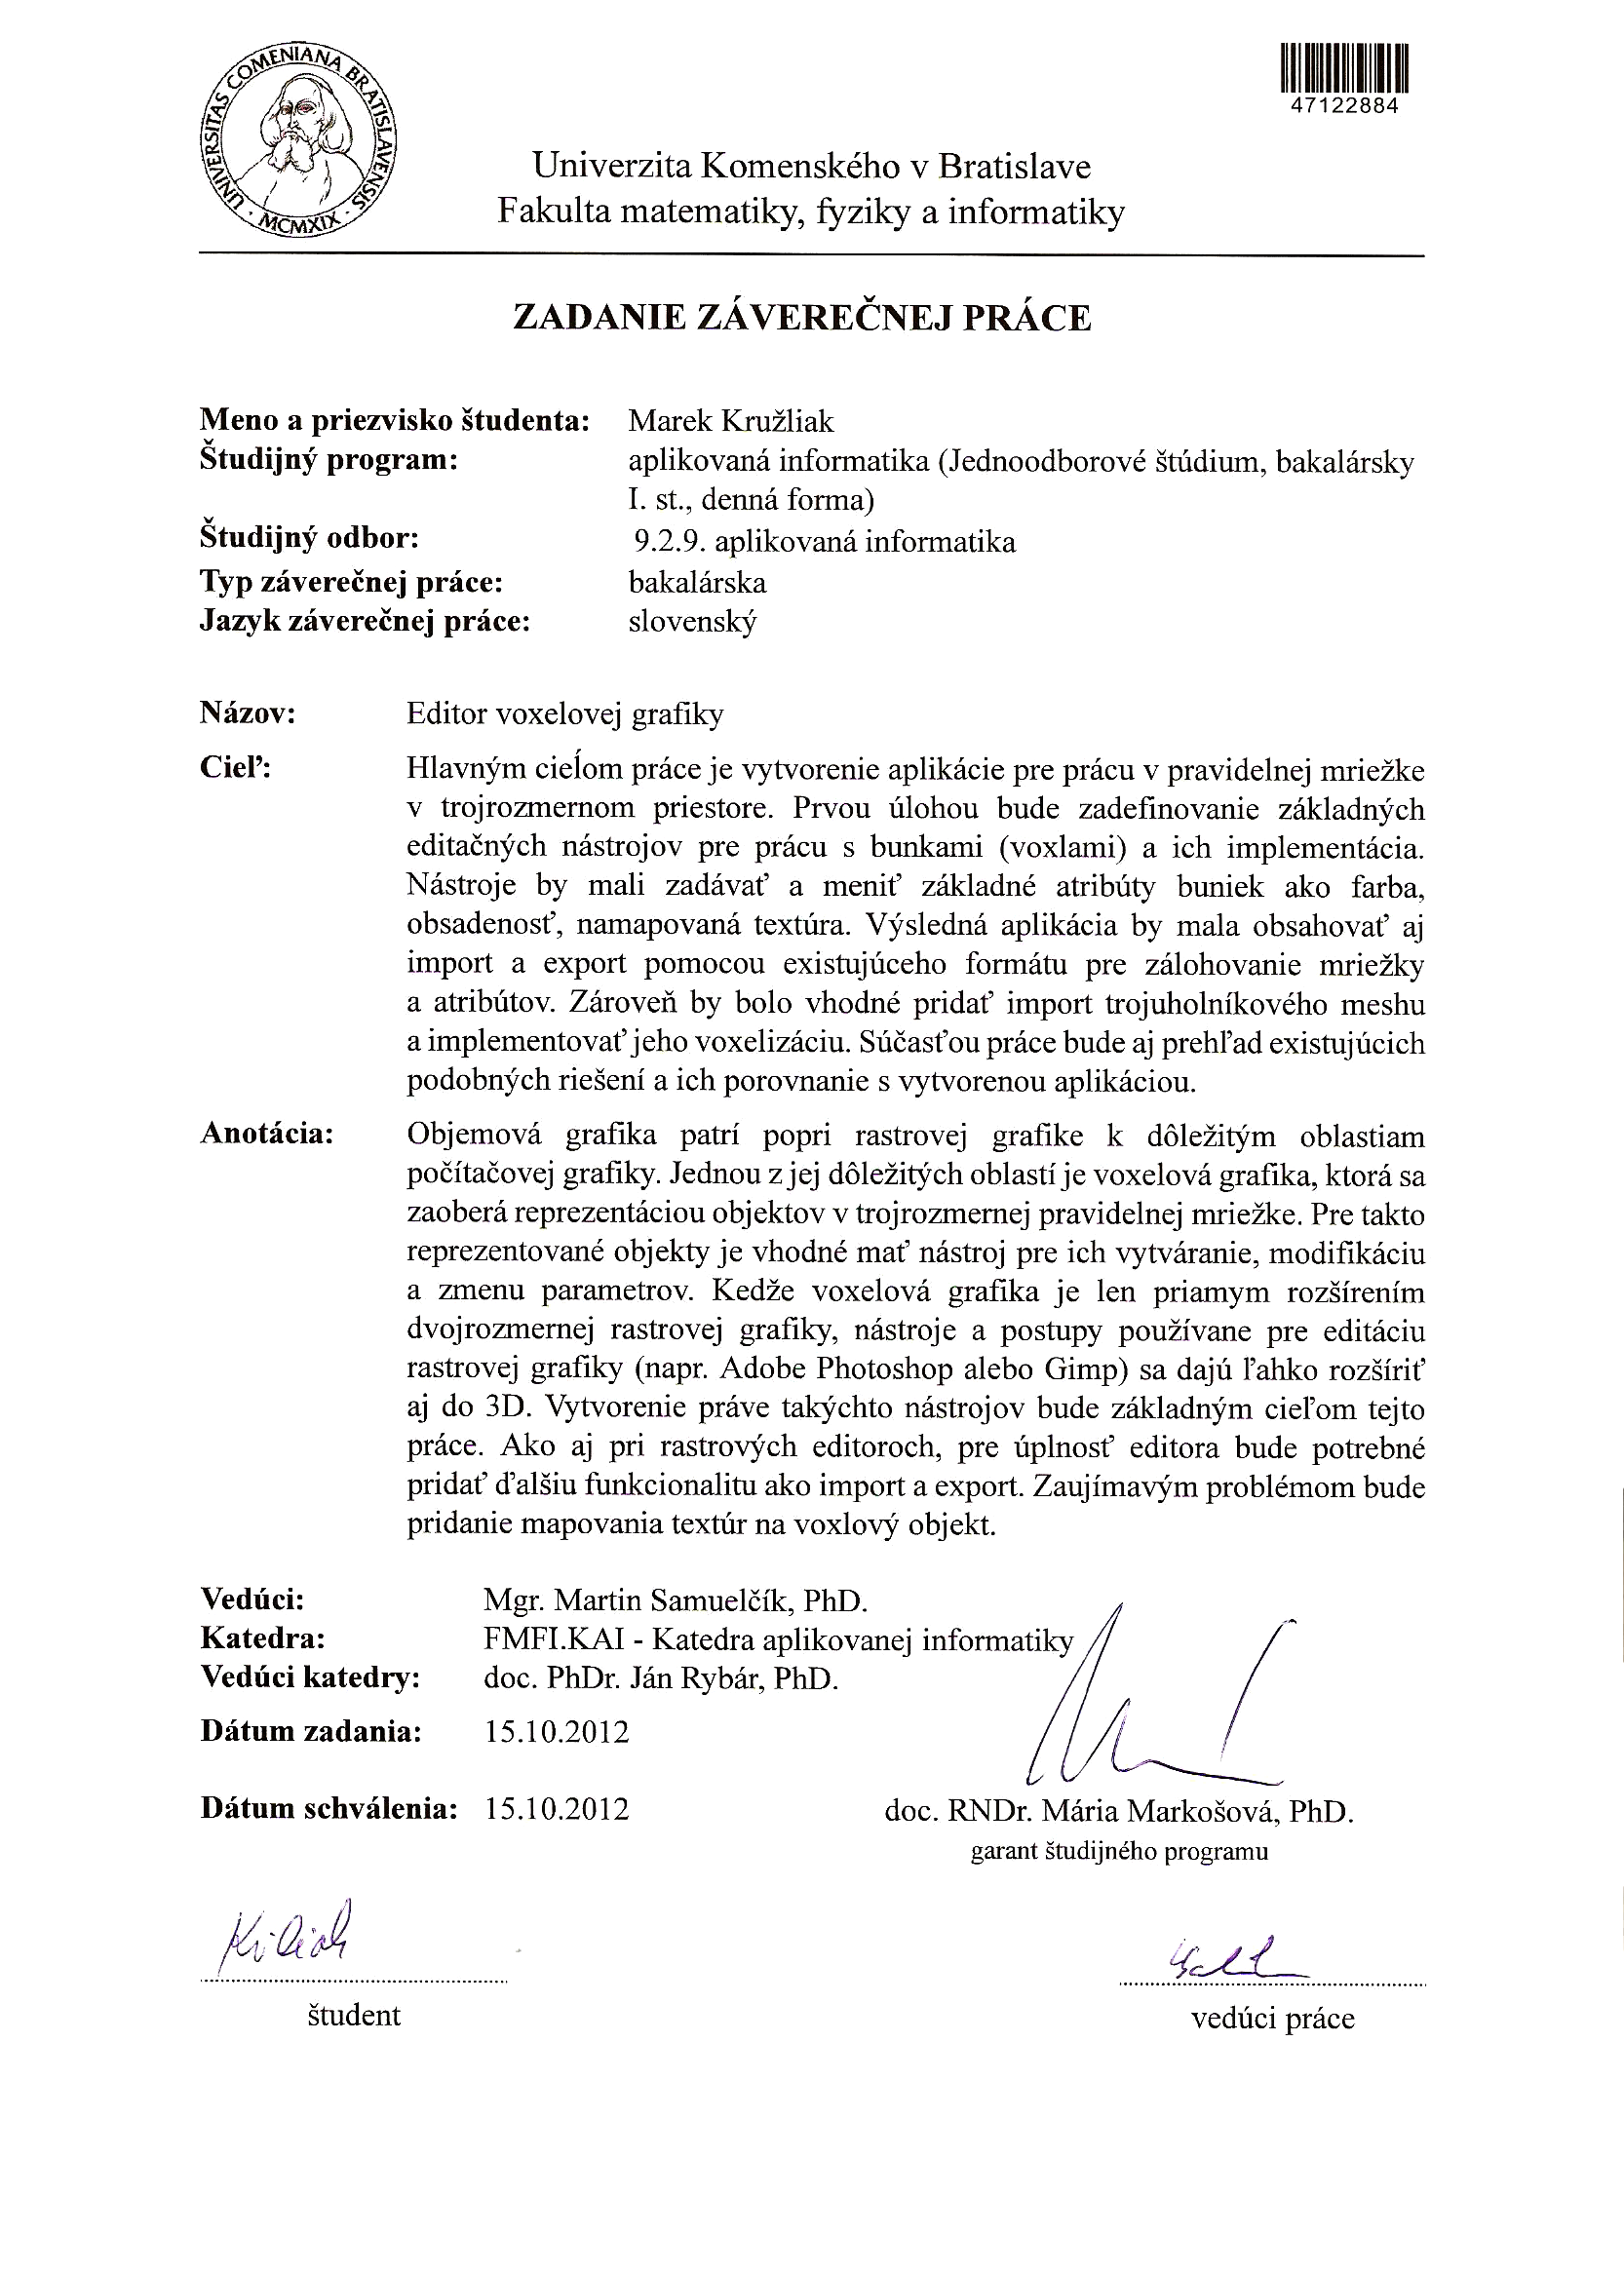
\includegraphics[width=597pt,height=845pt,keepaspectratio]{zadanie.png}}
\restoregeometry
%prehlasenie
\thispagestyle{empty}
\vspace*{\fill}
\hfill
\begin{minipage}{0.63\textwidth}
Čestne prehlasujem, že som túto bakalársku prácu vypracoval samostatne s použitím citovaných zdrojov.

\bigskip
	\begin{flushright}
	\begin{minipage}{0.5\textwidth}
	\dotfill
	\end{minipage}
	\end{flushright}
\end{minipage}\eject
% Podakovanie
\thispagestyle{empty}
\topskip0pt
\vspace*{\fill}
\hfill
\begin{minipage}{0.65\textwidth}
\vspace{0pt}\raggedright
Ďakujem RNDr. Martinovi Samuelčíkovi, PhD. za to, že sa
ujal vedenia mojej bakalárskej práce a za jeho cenné rady
pri programovaní a pri písaní práce. 
\end{minipage}
\vspace*{\fill}
\eject

\setcounter{page}{1}
\pagenumbering{Roman}
% abstrakt
\begin{Huge}
\textbf{Abstrakt}  \\
\end{Huge}

Primárnym cieľom práce je opísať návrh a implementáciu praktického nástroja na tvorbu 
a editovanie voxelových objektov a scén. 
V práci sa taktiež venujeme vysvetleniu základných pojmov objemovej grafiky a jej využitiu mimo vedeckej sféry, teda v moderných herných enginoch a podobne.
Ďalej uvádzame príklady existujúcich riešení v danej oblasti, ich kladné a záporné stránky, a následné
využitie získaných poznatkov z ich testovania.
Práca taktiež opisuje zaujímavé algoritmické problémy, ktoré sa počas tvorby práce vyskytli, ich riešenie a implementáciu opísaného riešenia.\\



\textbf{Kľúčové slová:} voxel , objemová grafika, voxelizácia
\eject

\begin{Huge}
\textbf{Abstract}  \\
\end{Huge}

Primary goal of this paper is to describe design and implmentation of voxel editing tool. We also describe basic concept of volume graphics and its usage in commercial sphere, like modern game engines, animation etc. Next we mention examples of already existing solutions in this field, their strong and weak points and their influence on this work. In this paper we also analyze intersesting algorithmic problems, which appeard during implementation phase. \\

\textbf{Keywords:} voxel, volume graphics, voxelization
\tableofcontents
%zoznam obrazkov a tabuliek
\listoffigures
\begingroup
\let\clearpage\relax
\listoftables
\endgroup
%zoznam skratiek
\eject
\begin{Huge}
\noindent\textbf{Zoznam skratiek} 
\end{Huge}


\begin{figure}[!h]
		\bigskip
		\bigskip
		\hspace{0.5cm}
		\begin{minipage}[h]{0.1\textwidth}
		  WRF \\
		  NCEP \\
		  NCAR \\
		  NWP \\
		  GFS \\
		  NAM \\
		  RUC \\
		  SREF \\
		  GEFS \\
		  ECMWF \\
		  NOAA \\
		  ESRL \\
		  AFWA \\
		  NRL \\
		  CAPS \\
		  LES \\
		  WMO \\
		  TOGA \\
		  ME \\
		  MFE \\
		  MAE \\
		  RMSE \\
		  MSE \\
		  TS \\
		  MAD \\
		  GUI \\
		  VBA \\
		  SAS \\
		  CAWCR \\
		  IDL \\
		  NCL \\
		  MET \\
		  DTC \\
		  EVS \\
		  HEP \\
		  MISE \\
		  KDE \\
		  IMS \\
		  HTML \\
		  SVG \\
		\end{minipage}
		\begin{minipage}[h]{0.8\textwidth}
		  Weather Research and Forecasting \\
		  National Centers for Environmental Prediction \\
		  National Center for Atmospheric Research \\
		  Numerical Weather Prediction \\
		  Global Forecast System \\
		  North American Mesoscale Forecast System \\
		  Rapid Update Cycle \\
		  Short Range Ensemble Forecast \\
		  Global Ensemble Forecast System \\
		  European Centre for Medium-Range Weather Forecasts \\
		  National Oceanic and Atmospheric Administration \\
		  Earth System Research Laboratory \\
		  Air Force Weather Agency \\
		  Naval Research Laboratory \\
		  The Center for Analysis and Prediction of Storms \\
		  Large eddy simulation \\
		  World Meteorological Organization \\
		  Tropical Ocean Global Atmosphere \\
		  Mean Error \\
		  Mean Forecast Error \\
		  Mean Absolute Error \\
		  Root Mean Square Error \\
		  Mean Square Error \\
		  Tracking Signal \\
		  Median Absolute Deviation \\
		  Graphical User Interface \\
		  Visual Basic for Applications \\
		  Statistical Analysis Software \\
		  Centre for Australian Weather and Climate Research \\
		  Interactive Data Language \\
		  NCAR Command Language \\
		  Model Evaluation Tools \\
		  Developmental Testbed Center \\
		  Ensemble Verification System \\
		  Hydrological Ensemble Prediction \\
		  Mean Integrated Square Error \\
		  Kernel Density Estimation \\
		  Integrated Monitoring System \\
		  Hypertext Markup Language \\
		  Scalable Vector Graphics \\
		  \end{minipage}
	\end{figure}
	
\begin{figure}[!h]
		\bigskip
		\bigskip
		\hspace{0.5cm}
		\begin{minipage}[h]{0.1\textwidth}
		  CSS \\
		  CSV \\
		  UML \\
		\end{minipage}
		\begin{minipage}[h]{0.8\textwidth}
		  Cascading Style Sheets \\
		  Comma Separated Values \\
		  Unified Modeling Language \\		 
		\end{minipage}
	\end{figure}	
	 
			  
			  
			  

\eject
\setcounter{page}{1} 
\pagenumbering{arabic}

\chapter{Úvod}
	
	
Vizualizácia informácií a vizuálna analýza dát sú dnes veľmi vyvíjaným a moderným odvetvím počítačovej grafiky. Aplikácie vizualizácie informácií sú rôzne od ... cez ... až po ... Úlohou vizualizácie informácií je v prvom rade využitie ľudských kognitívnych schopností pre lepšie porozumenie dát.

Svoje využitie našla aj v procese verifikácie predpovedných modelov počasia. Dnešné metódy verifikácie predpovedí sa sústreďujú na numerický popis výkonu jednotlivých predpovedných modelov pomocou rôznorodých štatistických metód. Vo výsledku sa dáta opisujú ďalšími dátami, avšak práve na vizualizáciu týchto dát sa kladie veľmi slabý dôraz.

V našej práci sme preštudovali používané štatistické metódy pre verifikáciu spojitých premenných, ktoré predpovedá model \textit{WRF}. Hlavným cieľom práce sa však stal návrh a implementácia vizualizačných techník špeciálne navrhnutých pre potreby verifikácie. Sústredili sme sa obzvlášť na to, aby sme ušetrili cenný vizuálny priestor bez straty potrebných informácií. Návrh vizualizácie vychádza ...
\chapter{Verifikácia predpovedných modelov počasia}

Verifikácia je proces, ktorý má overiť správnosť fungovania predpovedného modelu počasia. Z tohto dôvodu je nepostrádateľnou súčasťou meteorologického výskumu a taktiež celkového procesu predpovedania počasia. \cite{MET:MET52}
Ciele verifikácie môžeme rozdeliť do troch skupín: \textit{administratívne}, \textit{vedecké} a \textit{ekonomické}.
Medzi \textit{administratívne ciele} patrí monitorovanie úspešnosti predpovedania modelu a nasmerovanie užívateľov na jeho správnu konfiguráciu alebo voľbu iného modelu. \textit{Vedeckými cieľmi} sú identifikovanie a oprava slabín modelu a taktiež vylepšovanie predpovedí. \textit{Ekonomickými cieľmi} sú rozhodovanie, kam majú smerovať investície do výskumu a iné závažné ekonomické rozhodnutia. \cite{IntroToVerif}

%TODO co sa da secko verifikovat alebo take daco...
% Standard verification methods:
% 	Methods for dichotomous (yes/no) forecasts
% 	Methods for multi-category forecasts
% 	Methods for forecasts of continuous variables
% 	Methods for probabilistic forecasts 

\section{Predpovedný model počasia}

Už v 19. storočí vývoj termodynamiky na základe Newtonovskej fyziky vyvrcholil v ucelení množiny fundamentálnych princípov, ktoré riadia prúdenie plynov v atmosfére. 
Začiatkom 20. storočia sa o matematický prístup k predpovedaniu počasia najviac zaslúžili osobnosti ako Vilhelm Bjerknes alebo Lewis F.Richardson. Avšak na ďalší úspech, v tejto oblasti, sa muselo čakať až na vynájdenie prvých počítačov počas 2. svetovej vojny ako bol IAS alebo ENIAC. \cite{Origins}
Prvá úspešná predpoveď bola vykonaná v 50. rokoch minulého storočia a to hlavne vďaka práci Jula Charneyho.
Následný vývoj vo výpočtovej sile počítačov, používanie satelitných pozorovaní a vývoj samotnej meteorológie ako vedy zapríčinil, že je numerická predpoveď počasia (NWP) dnes najúspešnejším prístupom ako predpovedať počasie.  \cite{Golding}

Odvtedy vzniklo veľké množstvo modelov, ako sú napríklad GFS, NAM, RUC, WRF, SREF, GEFS, ECMWF, ALADIN a mnoho ďalších. Naša práca sa zameriava konkrétne na verifikáciu modelu \textit{WRF}. Taktiež pokračuje neustály vývoj aj vďaka novým modelovacím technikám, novým parametrizáciám, a zvyšovaniu výkonu výpočtových zdrojov.

\begin{figure}
	\centering
	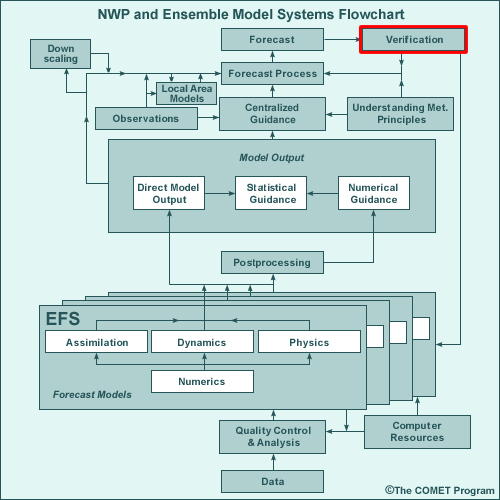
\includegraphics[width = 4in]{ForecastModelDiagramNew}
	\caption{Flowchart systému predpovedného model počasia od edukačného programu The COMET \cite{Comet}. Na obrázku je zvýraznená časť, ktorej sa venujeme v tejto práci.}
	\label{fig:fcstmodel}
\end{figure}

Ako môžeme vidieť na obrázku \ref{fig:fcstmodel} proces predpovedania počasia má okrem numerického modelu, ktorý je jej jadrom, aj iné časti. Ako príklad môžme spomenúť získavanie vstupných dát, ich predspracovanie, postprocesing, spracovanie výstupu a následne poskladanie samotnej predpovede. Cieľom nášho záujmu, celého procesu predpovedania, je \textit{verifikácia}. Ako môžme vidieť z obrázka, verifikácia vplýva na vyladenie parametrov modelu, avšak tento proces sa nedeje automaticky, ale vyžaduje prácu meteorológov a ich chápanie základných meteorologických princípov.


\subsection{WRF model}
\label{subsec:wrf}
Ako sme už spomenuli \textit{The Weather Research and Forecasting} (WRF) model je \textit{numerická predpoveď počasia} (NWP) a systém atmosferickej simulácie.

WRF je podporovaný, ako bežný nástroj pre univerzity, výskum a operačné komunity, pričom sa usiluje o splnenie požiadaviek ich všetkých súčasne.
Vývoj WRF modelu bol snahou mnohých spoločností ako napríklad \textit{The National Center for Atmospheric Research’s} (NCAR), \textit{Mesoscale and Microscale
Meteorology} (MMM), \textit{The National Oceanic and Atmospheric Administration’s} (NOAA) \textit{National Centers for Environmental Prediction} (NCEP) a \textit{Earth System Research Laboratory} (ESRL), oddelenie ministerstva obrany \textit{Air Force Weather Agency} (AFWA) a \textit{Naval
Research Laboratory} (NRL), \textit{The Center for Analysis and Prediction of Storms} (CAPS) \cite{WRF}. 

WRF model je vhodný pre širokú škálu aplikácií od \textit{metódy vzdušných vírov} (Large Eddy Simulation - LES) až po globálne simulácie počasia. Takéto aplikácie vyžadujú numerické predpovede v reálnom čase, vývoj a štúdium asimilácie dát, výskum parametrizovanej fyziky, výskum parametrizovanej fyziky ,modelovanie kvality ovzdušia, idealizované simulácie, čo všetko WRF model spĺňa.

V roku 2008 evidovala WRF viac ako 6000 užívateľov, no dnes (2014) eviduje viac ako 25000 užívateľov vo viac ako 130 krajinách sveta. Tieto fakty poukazujú na to, že WRF model má nie len veľkú základňu užívateľov, ale aj vývojárov a má v budúcnosti istotne svoje miesto a preto si myslíme, že sa oplatí investovať čas a úsilie do verifikácie tohto modelu.

\section{Dáta}
\label{sec:data}
Na správne zhodnotenie úspešnosti modelu potrebujeme dva druhy dát. V prvom rade sa jedná o dáta, ktoré sú výstupom z daného predpovedného modelu počasia, teda \textbf{predpovedané dáta}. Tieto umelo získané dáta chceme konfrontovať s realitou, aby sme si mohli vytvoriť obraz o správnom fungovaní celého modelu. Realitu v našom prípade predstavujú dáta namerané špecializovanými meteorologickými senzormi, ktoré označujeme ako \textbf{pozorované dáta} alebo skrátene \textit{pozorovania}.  

\subsection{Predpovedané dáta}
Predpovedané dáta z modelu WRF sa ukladajú vo formáte \textbf{GRIB}, čo je skratka pre \textit{GRIdded Binary} \cite{GRIB} alebo na iných miestach uvádzané ako \textit{General Regularly-distributed Information in Binary form} \cite{GRIB12}. Tento formát je štandardom Svetovej meteorologickej organizácie teda \textit{World Meteorological Organization} (WMO). Jedná sa o pomerne rozšírený formát, používaný pri veľkom množstve meteorologických aplikácií a je taktiež používaný ako výstupný formát pre iné predpovedné modely ako WRF, či už ECMWF, GFS, NAM, SREF alebo mnohé iné \cite{Products}.

Doteraz boli vyvinuté 3 verzie tohoto formátu od 0 po 2. Verzia 0 bola určená pre malé projekty typu TOGA a to iba s limitovaným použitím a dnes sa táto verzia už vôbec nepoužíva. Verzia grib 1 \cite{GRIB}, grib 2 \cite{GRIB12} sú dnes bežne používané väčšinou meteorologických centier.

Medzi verziami 1 a 2 nie sú žiadne rozdiely v obsahovej filozofii, preto popis obsahu gribovského formátu, ktorý tu uvádzame je spoločný pre obe tieto verzie. 
\textit{Gribovský súbor} (ďalej iba \textit{Grib}) pozostáva z viacerých \textit{Gribovských záznamov}, pričom jeden záznam môže existovať ako samostatný Grib. Vďaka tomu je možné ľahko spájať Griby, a to tiež v ľubovoľnom poradí, bez toho, aby sme ich nejako poškodili. Samozrejme musí byť zachovaná homogenita, čo sa týka verzií Gribov, teda verziu 1 nemožno miešať s verziou 2 a naopak.
Už samotný názov \textit{Gridded Binary} nám napovedá, že dáta sú usporiadané v pravidelnej mriežke. Každý Gribovský záznam obsahuje dvojrozmernú mriežku (zemepisná šírka x zemepisná dĺžka) hodnôt v určitom čase a vertikálnej hladine. Taktiež v hlavičke záznamu sa nachádzajú metainformácie, ktoré nám hovoria o aké dáta ide, teda o akú premennú sa jedná, čas predpovede, výškovú hladinu a podobne. Grib je zvyčajne z tohto dôvodu 2 až 5 rozmerná dátová štruktúra s veľkým množstvom veličín ako je napríklad teplota, tlak, relatívna vlhkosť, rosný bod, \textit{u} a \textit{v} súradnice vetra a ďalšie, ktoré sú definované v rôznych hladinách. Taktiež je dôležité povedať, že Grib zriedkakedy zachytáva povrch celej planéty, ale iba vymedzenú skúmanú oblasť - \textit{doménu}.

\subsection{Pozorované dáta}
Pozorovania sa získavajú meraním priamo v teréne pomocou špecializovaných meracích zariadení, ktoré sú súčasťou meteo staníc. Každá stanica môže obsahovať iné vybavenie, ku príkladu teplomer, zrážkomer, barometer, vetromer a im podobné \cite{WeatherStation}, ktorými môžme zachytávať informácie o rôznych skúmaných veličinách. 
%http://www.weathergraphics.com/dl/obsman.pdf
% http://en.wikipedia.org/wiki/Weather_station

Majoritná časť meraní sa deje pri povrchu zeme priamo na meteo staniciach a nazývajú sa \textit{surface} merania. Tieto merania najlepšie popisujú dianie v oblasti najväčšieho záujmu (biosfére), avšak neobsahujú informáciu o dianí v iných výškových hladinách. Pozorovania týchto hladín sa dejú pomocou \textit{radiosondy}, ktorá je pripojená k meteo balónu alebo vypustená z lietadla smerom k zemi. Takéto pozorovania sa nazývajú \textit{upper air} merania.

Narozdiel od predpovedaných dát, pozorované dáta nemajú štandardizovaný formát a zvyčajne sa ukladajú do databázy.
Aby sme zhrnuli charakteristiku týchto dát, jedná sa o niekoľko meraných veličín, nameraných v konštantných časových krokoch - napríklad každú minútu alebo každú hodinu - v jednom konkrétnom geografickom bode a zvyčajne pri povrchu zeme, teda ak sa nejedná o upper air merania, ktoré sa uskutočňujú v štandardných výškových hladinách, ktoré sa merajú v hPa.

\subsection{Párovanie dát}
\label{subsec:pairing}
%TODO novy pristup
Z predpovedného modelu a rovnako aj z merania získame veľké množstvo hodnôt. Aby sme mohli korektne porovnať predpovede s pozorovaniami, je nevyhnutné nájsť správne párovanie týchto hodnôt, teda zistiť, ktorú hodnotu porovnať s ktorou, aby sme získali zmysluplný výsledok.

Vždy sa snažíme nájsť správnu predpoveď pre pozrovanie a nie naopak.
% Vzhľadom na charakter dát sa 
Dôvodom je, že chceme skúmať vzťah predpovede s realitou a preto v párovaní musí byť zahrnutých čo najviac \textbf{meraných} hodnôt, ak nie všetky.

Každá pozorovaná hodnota, ktorú chceme spárovať má štyri kľúče podľa ktorých hľadáme pár: \textit{meraná veličina} (napríklad teplota), \textit{čas merania}, \textit{výšková hladina} a \textit{geografická poloha}.
Nájsť všetky hodnoty podľa kľúča meranej veličiny v Gribe je ľahké, keďže sa jedná o kategorickú premennú, teda môže nadobúdať iba určitý konečný počet hodnôt. Toto sa však nedá povedať o čase, hladine a polohe, ktoré sú spojitými premennými.
 
Pre čas pozorovania, čas predpovede a výškovú hladinu existujú štandardy, ktoré určujú v akých časoch resp hladinách sa robia merania a predpovede, čo nám uľahčuje prácu. Ak sa napriek tomu čas alebo hladina v Gribe nevyskytuje, tak pár vyhadzujeme z párovania. 

V prípade polohy zo samozrejmých dôvodov neexistuje žiaden štandard a hustota mriežky v Gribe nemôže byť nikdy tak veľká, aby poloha našej stanice vždy dopadla na presný bod mriežky. Z tohoto dôvodu získavame hodnoty z mriežky z okolitých bodov a to dvoma metódami \textit{Point-to-Grid} a \textit{Grid-to-Point} \cite{IntroToVerif}, ktoré sú znázornené na obrázku \ref{fig:pointmethods}. Jedná sa vlastne o dve interpolačné metódy. Point-to-Grid predstavuje metódu \textit{najbližší sused} (\textit{Nearest Neighbour}) a Grid-to-Point \textit{bilineárnu interpolačnú metódu}. 

Výber správnej metódy môže značne ovplyvniť výsledok. Dôvodom je, že môžu byť veľké rozdiely hodnôt v okolitých mrežových bodoch a tak, ak pomocou Point-To-Grid metódy získame nízku hodnotu, tak pomocou Grid-To-Point môžeme získať hodnotu omnoho väčšiu, vplyvom zvyšných troch bodov, ktoré vstúpili do interpolácie. Nemožno však jednoznačne povedať, ktorá z metód je lepšia, keďže obe môžu v istých prípadoch dávať lepšie výsledky. 

\begin{figure}
	\centering
	\begin{tabular}{ c c }
	\subfloat[Point-to-Grid]{\includegraphics[width = 2.5in]{PointtoGrid}} &
	\subfloat[Grid-to-Point]{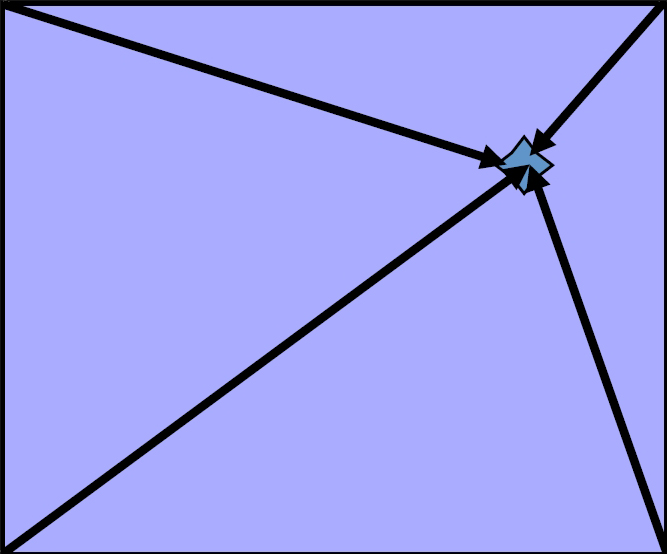
\includegraphics[width = 2.5in]{GridToPoint}} 
	\end{tabular}

	\caption{Vizuálne znázornenie dvoch bežne používaných metód na získavanie hodnôt z mriežky}
	\label{fig:pointmethods}
\end{figure}

\section{Meranie chyby predpovede}
\label{sec:errormeasurement}
Výsledkom procesu párovania je $n$ párov (predpoveď, pozorovanie), ktoré je možné porovnať. Z porovnania týchto dvojíc získame numerickú hodnotu, ktorá nám hovorí o veľkosti chyby predpovede daného modelu pre vybrané predpovedané časy.
\\
Chybu predpovede $e_i$ pre $i$-tu dvojicu $(y_i, \hat{y}_i)$ definujeme takto: 
\[  
	e_i = (y_i - \hat{y}_i)
\]
Kde $ y_i $ je predpoveď a $ \hat{y}_i $ je pozorovanie.
Takýmto spôsobom z $ n $ párov získame $ n $ chýb, ktoré agregujeme pomocou rôznych štatistických metód, ktoré sú bežne používané pri verifikácií predpovedí, ako sa spomína v \cite{RecommendOnVerif}, \cite{IntroToVerif} a \cite{ContinuousVerif}. Výsledkom agregácie je numerická hodnota, ktorá sa nazýva \textit{skóre} predpovede. 

\subsection{Stredná chyba predpovede}
Budeme ju označovať ako \textit{MFE} z anglického \textit{Mean Forecast Error}, ale v literatúre je možné ju nájsť ako \textit{ME} \cite{RecommendOnVerif}, teda \textit{stredná chyba} alebo ako \textit{Linear Bias} \cite{ContinuousVerif}, \cite{IntroToVerif}. Vzorec pre výpočet MFE vyzerá nasledovne:
\[
	MFE = \frac{1}{n}\sum\limits_{i=0}^{n}  e_i  
\]
MFE je možné vypočítať aj ako rozdiel priemerov predpovedí a pozorovaní.
\[
	MFE = \bar{y} - \bar{\hat{y}}  
\]
MFE vyjadruje priemerný smer chyby. To znamená, že pozitívny výsledok indikuje \textit{over-forecast}, teda nadhodnotenú predpoveď a negatívny výsledok \textit{under-forecast}, teda podhodnotenú predpoveď. Avšak MFE \textbf{nevyjadruje veľkosť} chyby v tomto smere, keďže kladné a záporné chyby sa navzájom môžu zrušiť. 
Napríklad máme množinu chýb $ E = \{2, -5\} $, tak MFE pre $ E $ je -1.5, ale priemerná veľkosť chyby je 3.5.  

\subsection{Stredná absolútna chyba}
Budeme ju označovať ako \textit{MAE} z anglického \textit{Mean Absolute Error}. Vzorec pre výpočet MAE vyzerá nasledovne:
\[
	MAE = \frac{1}{n}\sum\limits_{i=0}^{n} \lvert e_i \rvert 
\]
Narozdiel od MFE \textbf{neurčuje smer chyby}, ale vyjadruje veľkosť chyby. Z týchto dôvodov je v praxi odporúčané zobrazovať MFE a MAE súčasne \cite{RecommendOnVerif}. 

\subsection{Stredná kvadratická chyba}
Budeme ju označovať ako \textit{RMSE} z anglického \textit{Root Mean Square Error}. Vzorec pre výpočet RMSE vyzerá nasledovne:
\[
	RMSE = \sqrt{ \frac{1}{n}\sum\limits_{i=0}^{n} e_i^{2}  }
\]
Z povahy vzorca pre RMSE je jasné, že rovnako ako MAE, ani RMSE neurčuje smer chyby, pretože nadobúda vždy iba kladné hodnoty. 
Ďalšou vlastnosťou RMSE je, že nadobúda hodnoty vždy väčšie alebo rovné ako MAE, pričom výsledok RMSE je citlivý na veľké hodnoty chýb. \\
\label{subsec:mse}
V praxy sa zvykne používať aj \textit{MSE} (\textit{Mean Square Error}):
\[
	MSE = \frac{1}{n}\sum\limits_{i=0}^{n} e_i^{2} 
\]
Má podobné vlastnosti ako RMSE s jediným rozdielom, že RMSE meria veľkosť chyby zachovávajúc jednotky danej veličiny (napr. \textcelsius), zatiaľ čo MSE jednotky nezachováva \cite{RecommendOnVerif}. Preto sme si pre náš účel zvolili RMSE, ktoré je jednoduchšie zobraziť spolu s MFE a MAE v jednom grafe, keďže sa zachováva konzistentnosť jednotiek veličín.



%\subsection{Signál chybných predikcií}
%\[ 
%	TS = \frac{\sum\limits_{i=0}^{n} e_i}{MAE}
%\]

\subsection{Všeobecná kumulovaná chyba}
\label{subsec:cumulativeerror}
V našom systéme sme navrhli všeobecný vzorec na výpočet kumulovaného skóre, ktorým možno vyjadriť ľubovoľnú zo spomenutých štatistických metód. Takéto vyjadrenie umožňuje nie len všeobecnosť, ale aj jednoduché rozšírenie systému o ďalšie metódy a to nie len programátorom, ale aj samotným užívateľom systému.
\\
Všeobecný vzorec na výpočet \textit{skóre} pre danú predpoveď vyzerá takto:
\[
	Score = \Phi(\sum\limits_{i=0}^{n} \varepsilon(e_i))  
\]
Kde $ \Phi $ je ľubovoľná funkcia z $\mathbb{R}$ do $\mathbb{R}$, teda $ \Phi : \mathbb{R} \rightarrow \mathbb{R} $ a podobne funkcia $ \varepsilon : \mathbb{R} \rightarrow \mathbb{R} $.
Spomenuté metódy môžme teda skonštruovať zadefinovaním správneho $ \Phi $ a $ \varepsilon $. \\
Napríklad pre \textit{MFE}:
\[ \Phi(x) = \frac{x}{n} \]
\[ \varepsilon(e) = e \] 
Pre \textit{MAE}:
\[ \Phi(x) = \frac{x}{n} \]
\[ \varepsilon(e) = \lvert e \rvert \]
Pre \textit{RMSE}:
\[ \Phi(x) = \sqrt{\frac{x}{n}} \]
\[\varepsilon(e) = e^2 \]
Pre \textit{MSE}:
\[ \Phi(x) = \frac{x}{n} \]
\[ \varepsilon(e) = e^2 \] 

Ako sme spomenuli, je možné rozšírenie o ďalšie metódy a to napríklad o Brownov a Triggov \textit{signál chybných predikcií}, ktorý budeme označovať ako \textit{TS} z anglického \textit{Tracking Signal}. Tieto metódy sme vyššie nespomenuli, keďže sa v meteorologickej praxi nepoužívajú. Uvádzame ich však ako možné rozšírenie, keďže sú tieto metódy bežne používané pri verifikácii iných predpovedných modeloch, ako sú tie meteorologické.

\subsection{Medián absolútnych chýb}
\label{subsec:mad}
Budeme ju označovať ako \textit{MAD} z anglického \textit{Median Absolute Deviation}. Vzorec pre výpočet MAD vyzerá nasledovne:
\[
	MAD = median( \lvert e  \rvert) = \tilde{ \lvert e  \rvert}
\]
Nech je daná usporiadaná postupnosť $ Y_1, \ldots , Y_N $, tak potom $ median $ náhodnej premennej $ x $ je definovaný rovnako ako v \cite{StatMedian}:
\[
	median(x) = \tilde{x} \equiv \left\{
		\begin{array}{ll}
			Y_{(N+1)/2}  & \mbox{ak } N\mod{2} = 0 \\
			\frac{1}{2}(Y_{(N+1)/2} + Y_{(N+1)/2 + 1}) & \mbox{ak } N\mod{2} = 1
		\end{array}
	\right.
\]
Z daného vzorca môžeme vidieť podobné vlastnosti ako má MAE, avšak MAD je robustnejší a extrémne chyby nemajú na skóre žiaden efekt.

%TODO pridat LEPS - http://www.cawcr.gov.au/projects/verification/LEPS.php
% preto treba aj zmenit nejake veci 
\chapter{Predchádzajúce riešenia}

\section{Verifikačný softvér}

Verifikácia predpovedných modelov počasia je úloha dokonale stvorená pre automatizáciu. 
Z tohto dôvodu meteorológovia začali využívať dostupný štatistický softvér 
a neskôr boli taktiež vyvíjané špecializované nástroje určené pre verifikáciu.
Môžeme teda rozdeliť verifikačný softvér do dvoch základných kategórií a to \textit{štatistický} a \textit{špecializovaný}, ktorý je zväčša podporovaný rôznymi národnými a medzinárodnými organizáciami.

\subsection{Štatistický softvér}
%TODO
Spoločnou črtou: \\
	- obmedzená funkcionalita \\
	- obmedzená vizualizácia \\
	- slabé / žiadne GUI \\
	- vyžaduje znalosť špecifického programovacieho jazyka \\
	- ...


\subsubsection{Tabuľkový softvér}
Napriek tomu, že je tabuľkový softvér na výpočet štatistík zamietnutý komunitou vedcov a štatistikov ako nevhodný a neprofesionálny, tak je využívaný, a to pomerne často, aj vo vedeckých kruhoch. 
Výhodou je, že novému užívateľovi umožňuje okamžite vidieť všetky kroky v základných procedúrach verifikácie a teda je výborný pre výučbové účely. \cite{VerifSoft} 
Najznámejší kus softvéru z pomedzi komerčných produktov je \textit{Microsoft Excel}[ref] a z voľne dostupných je jeho opensoruce náprotivok \textit{Open Office Calculate}[ref]. Oba programy zahrňujú základné štatistické funkcie ako napríklad stredná kvadratická chyba (\textit{MSE}) pre spojité predpovede (pozri odsek \ref{subsec:mse}) a taktiež umožňujú generovanie jednoduchých grafov na základe tabuľkových dát. Tabuľkový softvér neposkytuje priamo funkcionalitu na výpočet ďalších sofistikovanejších verifikačných štatistík, avšak umožňuje ich implementáciu pomocou makro programovania v špecifickom jazyku. Pre Microsoft Excel je to \textit{Microsoft Visual Basic}[ref] a pre Open Office Calculate zasa \textit{OpenOffice.org Basic}[ref]. Oba jazyky patria do rodiny \textit{Basic} jazykov, takže majú mnoho podobných prvkov.  


\subsubsection{MATLAB}
\textit{MATLAB} je interaktívne prostredie s vlastným programovacím jazykom, ktorý je využívaný miliónmi inžinierov a vedcov po celom svete [ref] a tým nevynímajúc meteorológov a ďalších odborníkov pracujúcich v atmosférickom výskume. 
Zvyčajne sa MATLAB využíva na výskum a protoypovanie nových metód a procedúr \cite{VerifSoft}, pretože umožňuje rýchlu a jednoduchú implementáciu, keďže jeho súčasťou je mnoho matematických knižníc a je prispôsobený na prácu s maticami dát.
Výhodou MATLABU je, že umožňuje tvorbu GUI a taktiež poskytuje kreslenie rôznorodých grafov a diagramov.
Mali by sme však podotknúť, že podobne ako väčšina štatistického softvéru, aj \textit{MATLAB} je komerčný produkt. Jeho cena za jednu licenciu je \$2,650 (k roku 2015), čo je pomerne vysoká suma, ak vezmeme do úvahy za akým účelom chceme tento softvér využívať a ako dobre je naň prispôsobený.

\subsubsection{Minitab} % Toto tu netreba!



\subsubsection{R}

\subsubsection[SAS]{Statistical Analysis Software (SAS)}

\subsubsection[IDL]{Interactive Data Language (IDL)}

\subsection{Špecializovaný softvér}

\subsubsection[NCL]{NCAR Command Language (NCL)}

\subsubsection[MET]{Model Evaluation Tools (MET)}

\subsubsection[EVS]{Ensemble Verification System (EVS)}


%TODO tabuľka softvéru

\section{Vizualizácia verifikácie}

\subsection{Scatterplot}

\subsection{Boxplot}

\subsection{Time series plot}
\chapter{Návrh riešenia}


\section{Návrh systému}

\section{Návrh vizualizácie}

\subsection{Charakteristika dát}

\subsection{Špecifikácia požiadaviek na vizualizáciu}

\subsection{Návrh vizualizácie distribúcie chýb}
Pri verifikácii predpovede spojitej premennej sme použili štatistické metódy spomenuté v sekcii \ref{sec:errormeasurement}, ktorých výsledok sme následne vizualizovali. Pôvodné dáta však zostali skryté za použitým matematickým modelom, a tak sme stratili informáciu o distribúcii chyby. Pri verifikácii sa štandardne používajú dve metódy na priamu, či nepriamu vizualizáciu a analýzu distribúcie, ktoré sme opísali v sekcii \ref{sec:prevvis}. Týmito metódami sú bodový graf (pozri podsekciu \ref{subsec:scatterplot}) a krabicový diagram (pozri podsekciu \ref{subsec:boxplot}).

Pri návrh vizualizácie sme vyskúšali niekoľko vizualizačných techník a zvážili ich silné a slabé stránky. 

\subsubsection{Graf hustoty} %Density plot


\subsubsection{Pruhový kvantilový diagram} 
Z časti \ref{subsec:scatterplot} sme už dobre oboznámený s pojmom kvantil. Klasický kvantilový diagram zobrazuje kvantil hodnôt pre jednu dimenziu. Ak si vezmeme naše dáta, kde pre každý čas je niekoľko chýb predpovedí, tak kvantilový diagram skonštruujeme tak, že pre každý čas vypočítame kvantil, ktorý zobrazíme ako bod alebo ako súčasť lomenej čiary v grafe.
Prirodzeným rozšírením je zobrazovať nielen jeden kvantil, ale mnoho kvantilov súčasne. Zvyčajne sú to tieto kvantily $ Q_{0.02}, Q_{0.98}, Q_{0.25}, Q_{0.75}, Q_{0.5} $. V našej práci sme využili toto rozšírenie na lepšie zobrazenie distribúcie a navrhli sme takzvaný \textit{pruhový kvantilový diagram}.

Jeden \textit{pruh} v grafe definujeme pomocou dvojíc hodnôt v čase - spodným a jeho protiľahlým kvantilom. Spodným kvantilom je kvanitl $ Q_{\alpha} $ a k nemu protiľahlý je kvantil $ Q_{1 - \alpha} $, kde $ 0 \leq \alpha \leq \frac{1}{2} $. Vidíme teda, že pruh ohraničuje hodnoty v okolí stredu usporiadanej množiny dát. Špeciálnym prípadom pruhu je pre $ \alpha = \frac{1}{2} $, vtedy spodný aj horný kvantil je $ Q_{0.5} $, čo je vlastne medián.

Pri návrhu vizualizácie sme sa snažili, aby mohol mať diagram variabilný počet pruhov a taktiež, aby .... Tento problém sme vyriešili tak, že sme

% TODO obrázok a zrozumitelnejšie vysvetliť
Takto definovaný pruh sa potom vizualizuje, ako plocha medzi krivkami, ktoré tvoria dvojice hodnôt patriace danému pruhu.



%TODO toto musím ešte celé premyslieť!


\subsubsection{Funkčný krabicový diagram}
Pre pochopenie dát je dôležité, aby sme sa vedeli pozrieť na hodnoty v ich kontexte. Všetky predošlé techniky uvažovali o chybe ako o samostatnej hodnote pre určitý predpovedný čas, avšak chyby sa nenachádzajú len v kontexte predpovedného času, ale aj v kontexte konkrétnej predpovede. Preto môžme uvažovať o predpovediach ako o funkciách $ x_{i}(t) $, kde $ i \in \{1..n\}$ je poradie predpovede a $ t \in I $ je čas predpovede, kde $ I $ je časový interval predpovede z $ \mathbb{R} $ (v našom prípade sa jednalo o dvojdňovú, teda 48 hodinovú predpoveď).

Takýmto spôsobom sme sa dostali do novej situácie, kedy nechceme vizualizovať distribúciu jednotlivých chýb, ale celých predpovedí, ktoré chápeme ako funkcie. Na riešenie tohto problému existuje niekoľko spôsobov, z ktorých sme si zvolili \textit{funkčný krabicový diagram} \cite{FunctionalBoxplot}, keďže myšlienkovo vychádza z klasického krabicového diagramu, ktorý je jednak na túto situáciu vhodný ale je tiež medzi užívateľmi dobre známy a zaužívaný.

Ako sme spomenuli v časti \ref{subsec:boxplot}, klasický krabicový diagram potrebuje na svoju konštrukciu 5 hodnôt: 3 kvartily a 2 extrémy. Aby sme tieto hodnoty našli pre funkcie, musíme ich vedieť porovnať a povedať, ktorá je \textquotedblleft väčšia\textquotedblright alebo \textquotedblleft menšia\textquotedblright. Autori funkčného krabicového diagramu riešia problém s využitím takzvanej pásmovej hĺbky (\textit{band depth}) \cite{BandDepth}. Grafom $ G $ funkcie $ x $ je množina bodov $ G = \{ (t,x(t)) : t \in I \} $. Pásmo $ \mathcal{B} $ (\textit{band}) v $ \mathbb{R}^{2}  $ ohraničené krivkami $ x_{i_{1}}, x_{i_{2}}, .. , x_{i_{k}} $, kde $ k \geq 2 $ je definované takto:
\[
	\mathcal{B}(x_{i_{1}}, x_{i_{2}}, .. , x_{i_{k}}) = \{ (t,y) : t \in I, \min_{r=1..k}x_{i_{r}}(t) \leq y \leq \min_{r=1..k}x_{i_{r}}(t) \}
\]
Pásmo $ \mathcal{B} $ je teda množina všetkých bodov existujúcich medzi extrémami všetkých kriviek, ktoré doň vstupujú ako parameter. 
Pomocou týchto dvoch funkcií môžme definovať pomocnú funkciu $ BD_{n}^{(j)}(x) $ pre krivku $ x $, ktorá vyzerá takto:
\[
	BD^{(j)}_{n}(x) = {n \choose j}^{-1} \sum_{1 \leq i_{1} < i_{2} < ... < i_{j} \leq n} \mathcal{I}\{ G(x) \subset \mathcal{B}(x_{i_{1}}, ... ,x_{i_{j}}) \}, j \geq 2
\]
kde $ j $ je počet kriviek definujúce pásmo $ \mathcal{B} $, $ n $ je celkový počet kriviek a $ \mathcal{I} $ je takáto funkcia:
\[
	\mathcal{I}(x) = \left\{
	\begin{array}{ll}
	1 & \mbox{ak platí x}  \\
	0 & \mbox{ak neplatí x} 
	\end{array}
	\right.
\]
Pomocná funkcia $ BD $ pre krivku $ x $ definuje pomer všetkých pásem zložených z $ j $ kriviek, v ktorých sa graf $ G(x) $ nachádza, ku všetkým možným $ j $-ticiam kriviek vybraným z $ n $. 
Samotná funkcia pásmovej hĺbky $ \mathcal{BD} $ pre krivku $ x $ je definovaná takto:
\[
	\mathcal{BD}_{n, J}(x) = \sum_{j = 2}^{J} BD^{(j)}_{n}(x), J \geq 2
\]
Hĺbka pásma $ \mathcal{BD} $ je teda suma všetkých $ BD $ pre počet kriviek 2 až $ J $.

Autor článku definujúci pojem pásmová hĺbka navrhol taktiež flexibilnejšiu verziu s použitím pomocnej funkcie $ MBD $ (\textit{modified band depth}) \cite{BandDepth}. V pravom rade je potrebné zadefinovať si funkciu $ A $, ktorá určí všetky časové body, kedy sa krivka $ x $ nachádza v pásme $ B $.
\[
	A(x, B) = \{ t \in I : (t, x(t)) \in G(x) \wedge (t, x(t)) \in B \}
\]
V spomínanom článku autori využívajú alternatívnu definíciu funkcie $ A $, do ktorej vstupuje $ j + 1 $ kriviek. Jej význam zostáva rovnaký ako pri našej definícii, avšak náš prístup považujeme za jednoduchší a zrozumiteľnejší. S využitím \textit{Lebesguevoej miery} $ \lambda $ autori ďalej definujú funkciu $ \lambda_{r} $, ktorá nám dáva "pomer času, ktorý krivka strávi v pásme":
\[
	\lambda_{r}(A) = \dfrac{\lambda(A)}{\lambda(I)} 
\]
Nová pomocná funkcia $ MBD $ je definovaná nasledovne:
\[
	MBD^{(j)}_{n}(x) = {n \choose j}^{-1} \sum_{1 \leq i_{1} < i_{2} < ... < i_{j} \leq n} \lambda_{r}\{ A(x, \mathcal{B}(x_{i_{1}}, ... ,x_{i_{j}})) \}, j \geq 2
\]
Ak platí, že $ G(x) \subset \mathcal{B}(x_{i_{1}}, ... ,x_{i_{j}}) $, tak funkcia $ MBD $ sa degeneruje na $ BD $ \cite{FunctionalBoxplot}.

V našej aplikácii sme sa rozhodli, že budeme pásmo definovať pomocou iba dvoch kriviek, čo nám vzorec výrazne zjednodušilo. Taktiež to implikovalo fakt, že pri výpočte $ MBD $ nie je potrebné $ {n \choose j}^{-1} $, keďže berieme pásma zložené vždy z rovnakého počtu kriviek. Pre naše účely sme si taktiež zjednodušili funkciu $ \lambda_{r} $ na $ \lambda $, keďže nepotrebujeme vlastnosť tejto funkcie, ktorá dosahovala to, že $ MBD $ pre špeciálny prípad degeneruje na $ BD $. Po týchto úpravách výsledný vzorec pre naše $ \mathcal{BD}' $ vyzerá nasledovne:
\[
	\mathcal{BD}'_{n}(x) = \sum_{1 \leq i_{1} < i_{2} \leq n} \lambda\{ A(x, \mathcal{B}(x_{i_{1}},x_{i_{2}})) \}
\]
Teraz, keď sme úspešne definovali mieru, podľa ktorej môžme usporiadať funkcie resp. ich krivky, je veľmi ľahké skonštruovať funkčný krabicový diagram.

\paragraph{}
Nech sú naše funkcie predpovedí $ x_{1},.., x_{n} $ usporiadané zostupne podľa $ \mathcal{BD}' $. Potom krivka pre funkciu $ x_{1} $ má najvyššiu pásmovú hĺbku a predstavuje strednú hodnotu pre množinu funkcií, teda niečo podobné ako medián hodnôt pri krabicovom diagrame. Pri konštrukcii funkcionálneho diagramu nám taktiež pomôže koncept centrálneho regiónu \cite{Liu}. Centrálny región $ C $ pre 50\% kriviek je pásmo vytvorené z 50\% najhlbších kriviek, teda:
\[
	C_{0.5} = B(x_{1}, x_{2}, .., x_{\lceil n / 2 \rceil} )
\] 
Vidíme, že Centrálny región $ C_{0.5} $ zaobaľuje 50\% najhlbších kriviek, a teda sa jedná o akúsi analógiu pre medzikvartálový rozsah (IQR) v klasickom krabicovom diagrame (pozri sekciu \ref{subsec:boxplot}), ktorý ohraničoval 50\% centrálnych dát. Zobrazením hraničných bodov tohto regiónu získame obálku myšlienkovo totožnú boxu v krabicovom diagrame (pozri obrázok \ref{fig:functionalboxplot}b) ). Táto myšlienka sa dá použiť ďalej a môžme, tak ako na obrázku \ref{fig:functionalboxplot}c) , zobraziť taktiež 25\%-ný a 75\%-ný centrálny región $ C_{0.25} $, $ C_{0.75} $, avšak kvôli nižšej čitateľnosti grafu sme túto alternatívu nepoužili.

V prípade, že nepotrebujeme identifikovať \textit{outlier}-ov, tak extremálne hodnoty je už veľmi jednoduché získať, pretože ich tvorí pásmo zložené zo všetkých kriviek $ B(x_{1}, .., x_{n}) $. V opačnom prípade musíme najprv identifikovať \textit{outlier}-ov, ktorých potom vylúčime z výpočtov. Opäť sa využíva myšlienka z klasického krabicového diagramu, kedy sa \textit{outlier} určil pomocou hodnoty $ c \times IQR $, kde $ c $ bolo zvyčajne 1.5. Hranice sa teda získajú naškálovaním centrálneho regiónu so škálovacím faktorom 1.5 a všetky krivky, ktoré sa v tomto regióne nenachádzajú, budú považované za \textit{outlier}-ov. Test na \textit{outlier}-a vyzerá teda takto:
\[	y_{i}(t) = 1.5 \times x_{i}(t) \]
\[	isOutlier(x) = [ G(x) \nsubseteq B(y_{1},..,y_{\lceil n / 2 \rceil}) ] \]
Na obrázku \ref{fig:functionalboxplot}b) môžme vidieť červené prerušované čiary, ktorými sú \textit{outlier}-i znázornené.

V našej práci sme do diagramu pridali ešte jednu krivku pre ľubovoľnú štatistiku vypočítanú z chýb ako napríklad MFE, MAE alebo RMSE (pozri sekciu \ref{sec:errormeasurement}). Takto môžme spraviť porovnanie distribúcie chýb s vypočítanou štatistikou.
%TODO to je troška klamstvo ne?


\begin{figure}
	\centering
	\hspace*{-0.9in}
	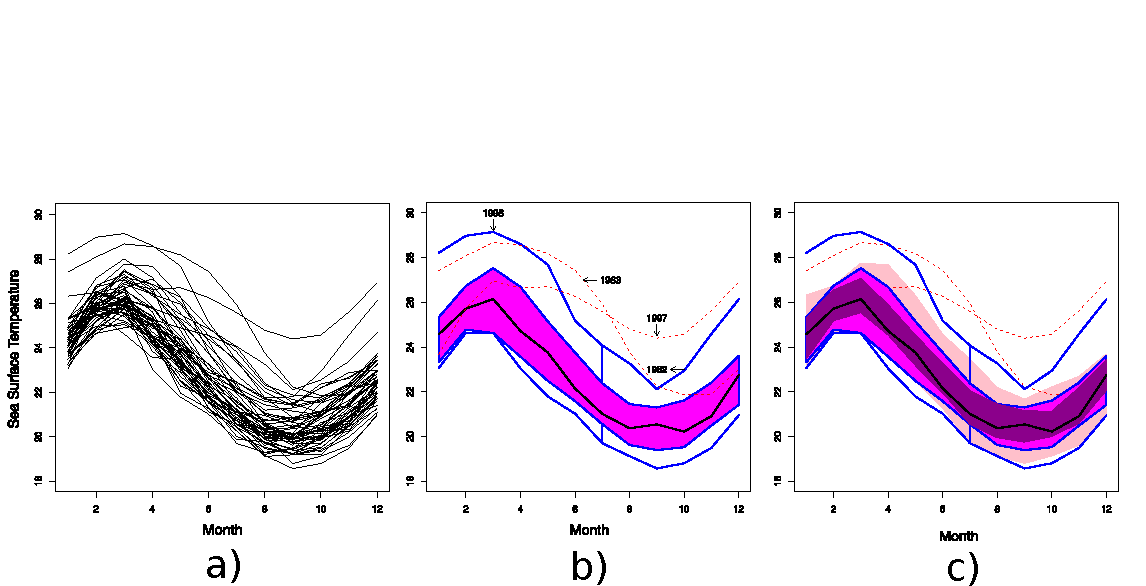
\includegraphics[width = 7.5in]{functionalboxplot}
	\caption{Obrázky z článku \textit{Functional Boxplots}  \cite{FunctionalBoxplot}  a) Funkcie meraní teploty hladiny mora b) Funkčný krabicový diagram c) Rozšírený Funkčný krabicový diagram o centrálne regióny $ C_{0.25} $ a $ C_{0.75} $ }
	\label{fig:functionalboxplot}
\end{figure}


%TODO obrazok pasmo

\subsubsection{Porovnanie metód}

Tu bude pekný obrázok a obkeci.


\subsection{Návrh farebnej palety}

\chapter{Implementácia}

\chapter{Výsledky}


\bibliographystyle{alpha}
\raggedright
\bibliography{literatura}


\end{document}
